%
% File acl2012.tex
%
% Contact: Maggie Li (cswjli@comp.polyu.edu.hk), Michael White (mwhite@ling.osu.edu)
%%
%% Based on the style files for ACL2008 by Joakim Nivre and Noah Smith
%% and that of ACL2010 by Jing-Shin Chang and Philipp Koehn


\documentclass[11pt,letterpaper]{article}
\usepackage[letterpaper]{geometry}
\usepackage{acl2012}
\usepackage{times}
\usepackage{latexsym}
\usepackage{amsmath}
\usepackage{amsfonts}
%\usepackage{cite}
% \usepackage[sort&compress]{natbib}
\usepackage{multirow}
\usepackage{graphicx}
\usepackage{url}
\graphicspath{ {images/} }
\makeatletter
\newcommand{\@BIBLABEL}{\@emptybiblabel}
\newcommand{\@emptybiblabel}[1]{}
\makeatother
\usepackage[hidelinks]{hyperref}
\DeclareMathOperator*{\argmax}{arg\,max}
\setlength\titlebox{6.5cm}    % Expanding the titlebox
\setlength{\thinmuskip}{0mu}
\setlength{\medmuskip}{0mu}
\setlength{\thickmuskip}{0mu} 

\title{Discrete Structured Representation Learning}

\author{Benjamin Striner \\
  {\tt bstriner@andrew.cmu.edu} \\}

\date{October 19, 2017}

\begin{document}
\maketitle
\begin{abstract}
Discrete structured representations are more understandable and explainable than continuous dense representations. Neural networks are efficient to optimize but do not allow for easy interpretation. We adapt a simple network to learn discrete hidden representations that can be interpreted as ontologies or decision trees. This provides a means to increase the interpretability and explainability of neural networks. We also examine conventional postmortem clustering and find that it frequently underperforms random clustering.
\end{abstract}

\section{Introduction}

Hidden representations inferred by neural networks are commonly dense and continuous. Continuous dense representations are hard to interpret, so techniques for clustering, visualization, and dimensionality reduction are applied to make hidden representations understandable \cite{Montavon}. These analyses are commonly applied `postmortem' (after training).

Traditional knowledge representations are structured and discrete, such as tables, trees, or networks. For example, knowledge can be represented by a network such as Wikipedia (which also contains tabular data), sentences can be diagrammed as networks, and logical proofs can be represented as trees. Conventional linguistic ontologies attempt to organize words, concepts, or other objects into discrete structures, such as hierarchical trees (\textit{e.g.}, WordNet, PropBank) \cite{Miller:1995:WLD:219717.219748}. These types of representation tend to be more understandable than neural networks.

We provide a method for expanding existing neural networks to learn discrete hidden representations. These models attempt to imitate naturally generated representations, which should be more interpretable and explainable.

Discrete representations are advantageous for formal higher-level logic and coding efficiency. For instance, a discrete symbol set may be required to implement a discrete logic system. This may explain why human knowledge is naturally represented as structured networks. In addition, discrete representations allow for radical reduction in the number of bits required to encode each input \cite{Hu17}.

First, this paper describes methods for learning a discrete representation, using a skipgram model as an example. Second, this paper describes a series of experiments comparing postmortem clustering to proposed methods. Finally, this paper discusses results, finding that proposed models effectively cluster the vocabulary, and that postmortem clustering frequently performs worse than random clustering.

\section{Method}

To focus on the core optimization problem, we experimented with one of the simplest models, a skipgram model as discussed in \cite{Mikolov1301} and \cite{MikolovSCCD13}.

We first examine properties of the distribution. Second, we explain common methods for continuous factoring. Third, we discuss methods for discrete and hierarchical factoring. Finally, we discuss forms of regularization that may be useful in training our models.

\subsection{Marginal and conditional entropy}

We examine the marginal and conditional entropy of a discrete distribution to determine the bounds on performance of factoring or clustering. We discuss methods for factoring the distribution $P(X,Y)$.

Let $X$ and $Y$ be discrete variables and let the matrix $A$ represent the joint distribution.

$$A_{x,y}=P(X=x, Y=y)$$

The entropy of the marginal distribution, $H(Y)$, measures the complexity of the data if only $Y$ is considered. In the case of a skipgram matrix, this is roughly the entropy of the unigram distribution.

\begin{align*}
h(x) &= -x \log(x) \\
P(Y=y) &= \sum_x P(X=x, Y=y) \\
H(Y) &=  \sum_y h(P(Y=y))
\end{align*}

The conditional entropy, $H(Y \mid X)$, measures the complexity of $Y$ if $X$ is known. A neural network trained given $X$ to predict $Y$ using cross-entropy loss will at best achieve this value. The conditional entropy is the joint probability times the negative log of the conditional probability, or alternatively the marginal probability times the entropy of the conditional distribution.

$$H(Y \mid X)=-\sum_{x,y} P(X, Y) \log(P(Y \mid X)) $$
$$P(X,Y) = P(X) P(Y \mid X)$$
$$H(Y \mid X)= \sum_{x,y}  P(X) h(P(Y \mid X))$$

The function $f(x)=-x \log(x)$ is concave. The entropy of a linear combination of distributions is greater than or equal to the linear combination of the entropy of the distributions. The entropy of the marginal distribution is greater than or equal to the conditional entropy.

\subsection{Continuous factoring}

A common method of continuous factoring is to embed each input into a continuous representation. A neural network is used to parameterize an approximation to the conditional distribution, $\tilde{P}(Y \mid X)$. The loss, $J$, is the expected conditional negative log likelihood (\textit{e.g.}, \cite{MikolovSCCD13} and \cite{Mikolov1301}).

A simple version of this model is parameterized by embeddings ($U$), weights ($W$) and bias ($b$) and uses a softmax to squash the outputs.

$$ \tilde{P}(Y\mid X) = \operatorname{softmax}(U W+b)$$
$$ J = -\sum_{x, y} P(Y,X) \log \tilde{P}(Y \mid X) $$
$$ J = -\mathbb{E}_{[x,y \sim X, Y]} \log \tilde{P}(Y \mid X) $$

\subsection{Discrete factoring or clustering}

A common practice for producing discrete clusters is to train a neural network and then apply clustering techniques to the learned continuous hidden space. Common clustering techniques include GMM and $k$-means \cite{Lloyd:2006:LSQ:2263356.2269955}. We examine how much information is actually retained by applying clustering to learned embeddings. We also examine methods to directly cluster inputs with respect to a given loss function.% Add more citations for clustering

If inputs in a dataset are clustered, the single output that minimizes the loss for a given cluster may be calculated analytically or iteratively. In the case of minimizing entropy, constrained by the space of valid distributions, the analytic solution is straightforward.

$$\min_{\tilde{x}}[\sum_i-x_i \log(\tilde{x_i})] = x$$

The expected conditional negative log likelihood is the conditional entropy of the combined distributions, analogous to the neural network loss discussed above. Similar approaches could be applied to more complicated neural networks, but a simple conditional distribution is sufficient to analyze the core problem of learning discrete representations.

Let $X$ be clustered into a discrete space $Z$. Let $C$ be an indicator matrix where $C_{z,x}$ indicates that $X=x$ is a member of $Z=z$. $C$ encodes the distribution $P(Z \mid X)$. $C$ is constrained to a valid indicator matrix. The joint distribution $B_{z,y}=P(Y=y,Z=z)$ can be calculated by the dot product between the indicator and $P(Y,X)$. Note that $Z$ and $Y$ are independent given $X$.

$$P(Z \mid X,Y) = P(Z \mid X)$$
$$P(Y,Z) = \sum_x P(Y,X) P(Z \mid X)$$
$$B = C A $$ 

If the inputs $X$ are encoded discretely into $Z$ where $Z$ is overfull, some information is lost.  The matrix $B$, $P(Y,Z)$, is a linear combination of rows of the matrix $A$, $P(Y,X)$. Therefore $H(Y \mid Z) \ge H(Y \mid X)$ due to the concavity of $h$. 

By relaxing the constraints on $C$, we can create a parameterization of $P(Z \mid X)$ that allows for gradient descent on the conditional entropy $H(Y\mid Z)$. A simple parameterization
is $C=\operatorname{softmax}(W)$. If the softmax is fully saturated, each input, $X$, will be assigned to one and only one cluster, $Z$. At initialization, each row is assigned to a random mixture of clusters. The softmax ensures that $C$ may be validly interpreted as $P(Z \mid X)$. By the concavity of $h$, we predict that the model will tend towards saturation. A mixture of distributions will have a higher entropy than the component distributions.

$$ J = H(Y \mid Z) $$
$$ J = - \sum_{y,z} P(Y, Z) \log( P(Y \mid Z)) $$

For more complicated models, it may become necessary to approximate $P(Y \mid Z)$ with a neural network as well. In that case the following formulation may be more useful. The two parameterized values are $\tilde{P}(Y \mid Z)$ and $P(Z \mid X)$.

$$ J = - \sum_{y,z,x} P(Y, Z) P(Z \mid X) \log( \tilde{P}(Y \mid Z)) $$
$$ J = - \mathbb{E}_{x,y \sim X, Y} \sum_{z} P(Z \mid X) \log( \tilde{P}(Y \mid Z)) $$

\subsection{Hierarchical clustering}

The simplest discrete structured encoding is a binary tree. The address of a node in a binary tree of depth $d$ may be represented as a vector of $d$ bits. A complete binary tree will contain $2^d$ leaves at the base of the tree.

A reasonable objective for hierarchical clustering is the weighted sum of the conditional entropy of the clusters at each layer of the tree. If the learned representation is interpreted as a decision tree, the Bellman equation would suggest an exponential series as natural choice of weighting \cite{bellman1954}.

Let $Z_0,...,Z_d$ be the binary address of $X$ in the tree starting with $Z_0$ at the root.

$$ J = \sum_d \beta ^ d  H(Y \mid Z_0,\ldots, Z_d) $$

Intuitively, one is optimizing a weighted sum of how much information is available given the depth ($d$) of the tree or how many bits of the representation are provided. The parameter $\beta$ controls the importance of accuracy given few bits versus accuracy given many bits. This model attempts to pack more information into early bits and remaining differentiation into later bits. The meaning of the later bits is dependent on the earlier bits but the converse is not true.

We parameterize leaves at at the bottom layer of the tree $C_d$. We calculate the membership of nodes at previous layers $C_0,...,C_{d-1}$ by summing component leaves into parent nodes. We calculate the weighted loss over tree depth as described above.

\subsection{Regularization}

We experimented with several forms of regularization to examine the effects of regularization choice and weight on the performance of each model.

$L_1$ regularization penalizes the sum of the absolute values of the weights.

$$L_1(W) = \sum_{i,j} \lvert W_{i,j} \rvert $$

$L_2$ regularization penalizes the sum of the squares of the weights.

$$L_2(W) = \sum_{i,j} (W_{i,j})^2 $$

The exclusive lasso regularizer models the scenario when variables in the same group compete with each other and has been proven successful for inducing sparsity
\cite{zhou10a}, 
\cite{bach2012},
 \cite{Campbell15}.

$$V(W) = \sum_i (\sum_j \lvert W_{i,j} \rvert)^2$$ 

In order to ensure that the model fully utilizes all of the available clusters, we created a regularizer that prevents the marginal probability of any cluster from going to zero. We chose a logistic barrier regularizer applied to the marginal cluster probability. This regularizer approaches infinity as the expected probability of any cluster approaches zero.

$$ R(P) = -\sum_z \log[ \mathbb{E}_{x \sim \operatorname{unif}(X)} P(Z=z \mid X=x)]$$ 

We also performed experiments using $\mathbb{E}_{x \sim X}$, but this performed poorly in comparison to the expectation drawing from a uniform distribution.

$$R_0(P) =  -\sum_z \log [ \mathbb{E}_{x \sim X} P(Z=z \mid X=x) ]$$ 
$$R_0(P) =  -\sum_z \log P(Z=z )$$ 

\section{Experiments and Results}

We describe experiments and results factoring vocabulary from the Brown corpus. All source code and results are available online.\footnote{[Insert link to github]}

\subsection{Data preparation}

We calculated a skipgram matrix on which to perform our experiments from the Brown corpus. First, we cleaned the corpus by removing all non-alphabetic characters and capitalization and replacing words that appeared fewer than 20 times with a special `unknown' symbol, resulting in a set of $n=4,946$ symbols. Then, we then enumerated all symbols within a $k$ word window around each symbol to produce a list of skipgrams ($k$=3). Finally, we calculated the joint distribution by tabulating these skipgrams into a $n$ by $n$ matrix.

The entropy of the marginal distribution created from our matrix is 5.913 and the conditional entropy of the matrix is 5.326. Any reasonable factorization of the matrix should result in performance somewhere between those two values. These two values bound the results of all other experiments.

\subsection{Random clustering}

We assessed an initial baseline by randomly and uniformly assigning words to clusters. As expected, as the number of clusters increased, the conditional entropy of the output given the cluster decreased (Figure \ref{f:random}). Given two clusters, the mean conditional entropy is 5.9109 ($\sigma=0.0004$). Given 1024 clusters, the mean conditional entropy is 5.5664 ($\sigma=0.0018$).

\begin{figure}
  \caption{Random uniform clustering}
\label{f:random}
  \centering
    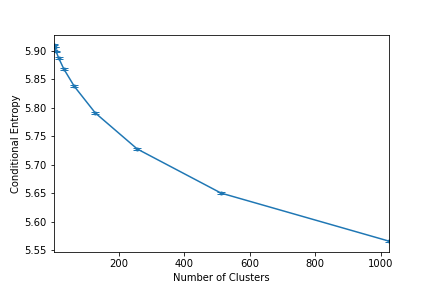
\includegraphics[width=0.5\textwidth]{random.png}
\end{figure}

\subsection{Skipgram models}

We trained unregularized continuous skipgram models varying the number of hidden units and found that performance asymptotically approached the analytically calculated conditional entropy (Figure \ref{f:baseline}). 

\begin{figure}
  \caption{Continuous skipgram model}
\label{f:baseline}
  \centering
    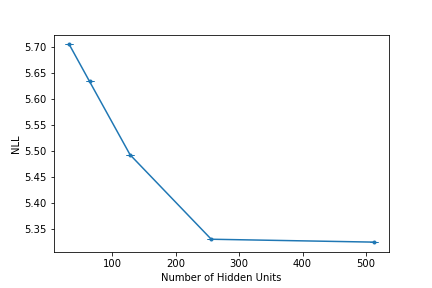
\includegraphics[width=0.5\textwidth]{baseline.png}
\end{figure}

We additionally trained models with $L_1$ and $L_2$ regularization. We used these models to examine how regularization and the number of hidden units affect the quality of post-mortem clustering. 

\subsection{Single-bit encoding}

We trained our model to discretely factor the matrix into 2 clusters of words. The mean conditional entropy of the resulting matrix was 5.8856 ($\sigma=4.4e-08$). This outperforms both the random baseline and any iteration of postmortem clustering. Additionally, the standard deviation of this model is roughly five orders of magnitude below most of the postmortem clusterings.

We clustered the hidden representations learned by each of our continuous skipgram models into 2 groups using Gaussian Mixture Model (GMM) clustering (Figure \ref{f:bgmm}) and k-means clustering (Figure \ref{f:bkm}). The best performance of any postmortem binary clustering trial was 5.8923. Many trials performed at or worse than random. GMM only performed better than random when a large number of hidden units were used. $k$-means clustering performed better than random and GMM when a small number of hidden units were used.

\begin{figure}
  \caption{Binary GMM clustering}
\label{f:bgmm}
  \centering
    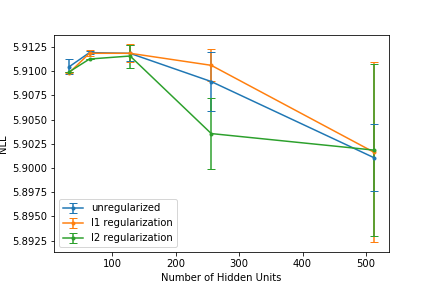
\includegraphics[width=0.5\textwidth]{binary_gmm.png}
\end{figure}

\begin{figure}
  \caption{Binary K-means clustering}
\label{f:bkm}
  \centering
    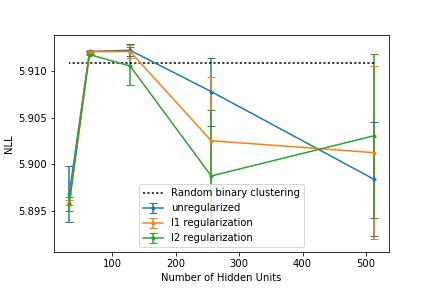
\includegraphics[width=0.5\textwidth]{binary_km.png}
\end{figure}

\subsection{Ten-bit encoding}

We trained our model to cluster the vocabulary into 1024 groups. The mean conditional entropy of the resulting clusters was 5.5480 ($\sigma=0.0008$), outperforming random clustering and postmortem clustering. The model accomplished this performance without utilizing all clusters; some clusters did not have any vocabulary assigned. The average utilization (out of 1024 clusters) was 809.4 ($\sigma=4.8$). We experimented with using regularization to increase the average utilization.

We experimented with the discussed barrier (Figure \ref{f:fb}), exclusive lasso (Figure \ref{f:fel}), $L_1$ (Figure \ref{f:fl1}), and $L_2$ (Figure \ref{f:fl2}) regularizers to determine the effect regularizer choice and weight has on conditional entropy and utilization. The barrier and exclusive lasso regularizers achieve similar performance, 5.5175 and 5.5166 respectively. Both appear effective at increasing utilization. The L1 regularizer was effective at increasing utilization but caused poor clustering. The L2 regularizer causes overall decreased clustering performance.

\begin{figure}
  \caption{Uniform Prior Regularization ($k=1024$)}
\label{f:fb}
  \centering
    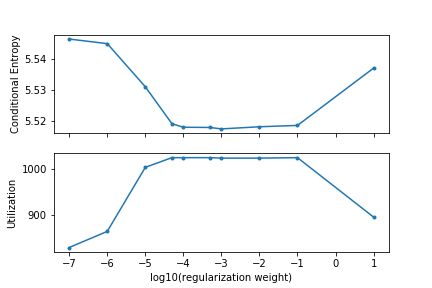
\includegraphics[width=0.5\textwidth]{skipgram_flat_b.png}
\end{figure}
\begin{figure}
  \caption{Exclusive Lasso Regularization ($k=1024$)}
\label{f:fel}
  \centering
    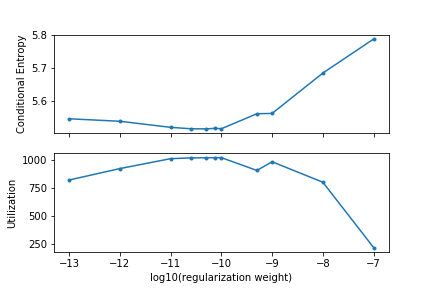
\includegraphics[width=0.5\textwidth]{skipgram_flat_el.png}
\end{figure}
\begin{figure}
  \caption{L1 Regularization ($k=1024$)}
\label{f:fl1}
  \centering
    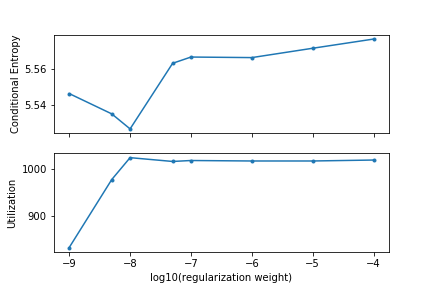
\includegraphics[width=0.5\textwidth]{skipgram_flat_l1.png}
\end{figure}
\begin{figure}
  \caption{L2 Regularization ($k=1024$)}
\label{f:fl2}
  \centering
    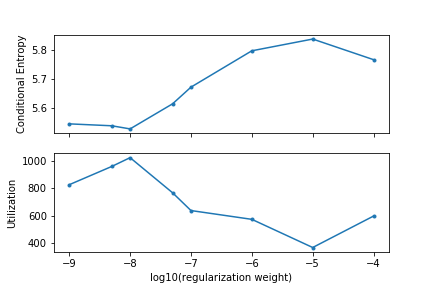
\includegraphics[width=0.5\textwidth]{skipgram_flat_l2.png}
\end{figure}

We clustered the hidden representations learned by each of our continuous skipgram models into 1024 groups using GMM clustering (Figure \ref{f:fgmm}), $k$-means clustering (Figure \ref{f:fkm}) and balanced hierarchical GMM (HGMM) clustering (Figure \ref{f:fbgmm}.\footnote{Balanced HGMM was implemented by fitting a binary GMM, sorting by $\log(P(A))-\log(P(B))$, splitting the vocabulary in half, and then recursively applying the same steps.} The best performance of any postmortem clustering with $k=1024$ using GMM or $k$-means was 5.59504.

Both GMM and $k$-means show clearer trends with $k=1024$ than $k=2$. Without regularization, small numbers of hidden dimensions cluster better than large numbers of hidden dimensions. With regularization, small and large numbers of hidden dimensions cluster better than a medium number of hidden dimensions.

Both GMM and $k$-means reliably perform worse than random uniform clustering. Balanced HGMM is able to perform as well as random under some hyperparameter settings.

\begin{figure}
  \caption{GMM clustering ($k=1024$)}
\label{f:fgmm}
  \centering
    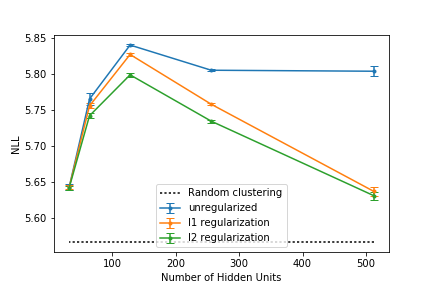
\includegraphics[width=0.5\textwidth]{flat_gmm.png}
\end{figure}

\begin{figure}
  \caption{$k$-means clustering ($k=1024$)}
\label{f:fkm}
  \centering
    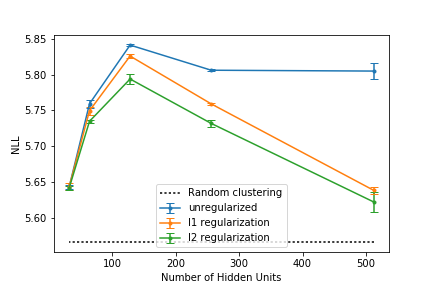
\includegraphics[width=0.5\textwidth]{flat_km.png}
\end{figure}

\begin{figure}
  \caption{Balanced HGMM clustering ($k=1024$)}
\label{f:fbgmm}
  \centering
    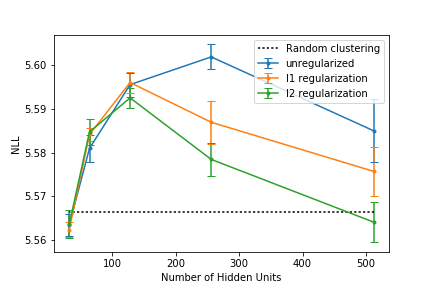
\includegraphics[width=0.5\textwidth]{flat_bgmm.png}
\end{figure}

\subsection{Binary tree clustering}

We trained binary trees of depth 10 so as to compare to our flat models of 1024 ($2^{10}$) clusters.

We varied $\beta$ to analyze the effect of the Bellman decay parameter (Figure \ref{f:beta}). Increasing $\beta$ produces better performance at deeper levels of the tree but worse performance near the root of the tree, and vice versa.

\begin{figure}
  \caption{Effect of Beta Hyperparameter}
\label{f:beta}
  \centering
    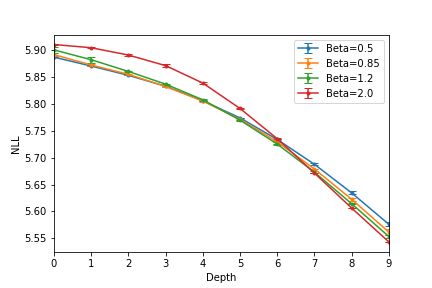
\includegraphics[width=0.5\textwidth]{skipgram_tree.png}
\end{figure}

Adding regularization to our binary tree model improved performance at the bottom of the tree while only slightly impacting performance at the top of the tree. For example, see Figure \ref{f:btb} and \ref{f:btel} for the effect of barrier and exclusive lasso regularization weight given $\beta=0.85$. It is impossible to identify a single `best' model, as the best choice of $\beta$ depends on the intended application.

\begin{figure}
  \caption{Binary tree with barrier regularizer ($\beta=0.85$)}
\label{f:btb}
  \centering
    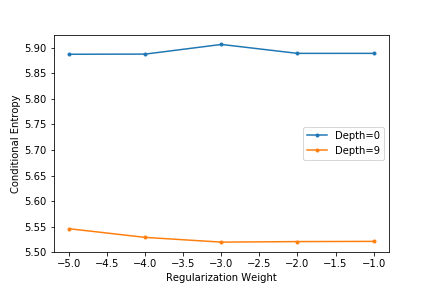
\includegraphics[width=0.5\textwidth]{skipgram_tree_b_0.png}
\end{figure}
\begin{figure}
  \caption{Binary tree with exclusive lasso regularizer ($\beta=0.85$)}
\label{f:btel}
  \centering
    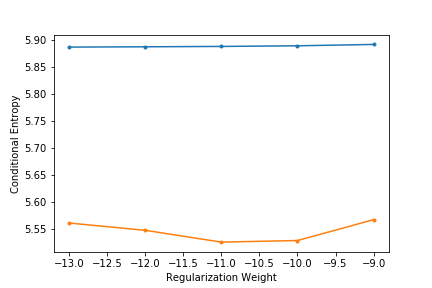
\includegraphics[width=0.5\textwidth]{skipgram_tree_el_0.png}
\end{figure}

\section{Discussion}

Optimizing the conditional entropy of $P(Y\mid Z)$ was an effective method of forming clusters. Clusters contained more information regarding $Y$ than clusters created using postmortem methods.

Regularization prevented under-utilization caused by death of some clusters. Barrier and exclusive lasso regularizers most effectively prevented under-utilization. It is critical to fully understand the dynamics of the optimization problem in such a simple environment, so it can be applied to more complicated networks.

Although clustering hidden representations should intuitively capture information related to the objective, we found that this was frequently not the case. Postmortem clustering was frequently worse than random clustering. Regularization and the size of the hidden space have strong effects on the result of the clustering, which can be avoided by using our proposed models.

For large numbers of clusters, postmortem methods actually reliably performed worse than random clustering. This unexpected result should caution against using postmortem clustering to help visualize continuous representation.

\section{Conclusion}
Discrete structured representations are natural and understandable. There are many challenges involved in adapting a model to learn discrete representations, above and beyond challenges intrinsic to the model. Learning a knowledge representation comparable to a traditional semantic ontology like WordNet or PropBank will require both datasets containing semantic content and a data structure and model capable of representing the complexities of semantic relationships.

These experiments address the simplest possible ontology, a binary tree. Even such a simple model can be interpreted as a decision tree, and is more explainable and understandable than a dense calculation. Further systems for discrete optimization should enable a higher class of structures, potentially able to represent discrete logic.

\bibliography{tacl}
\bibliographystyle{acl2012}


\end{document}



